%Notes by Harsh Mistry 
%Econ 301
%Based on Template From  https://www.cs.cmu.edu/~ggordon/10725-F12/template.tex

\documentclass[twoside]{article}
\setlength{\oddsidemargin}{0.25 in}
\setlength{\evensidemargin}{-0.25 in}
\setlength{\topmargin}{-0.6 in}
\setlength{\textwidth}{6.5 in}
\setlength{\textheight}{8.5 in}
\setlength{\headsep}{0.75 in}
\setlength{\parindent}{0 in}
\setlength{\parskip}{0.1 in}
\usepackage{amsmath,amsfonts,graphicx, color}
\newcounter{lecnum}
\renewcommand{\thepage}{\thelecnum-\arabic{page}}
\renewcommand{\thesection}{\thelecnum.\arabic{section}}
\renewcommand{\theequation}{\thelecnum.\arabic{equation}}
\renewcommand{\thefigure}{\thelecnum.\arabic{figure}}
\renewcommand{\thetable}{\thelecnum.\arabic{table}}
\newcommand{\lecture}[4]{
   \pagestyle{myheadings}
   \thispagestyle{plain}
   \newpage
   \setcounter{lecnum}{#1}
   \setcounter{page}{1}
   
   
%Info Box 
   \begin{center}
   \framebox{
      \vbox{\vspace{2mm}
    \hbox to 6.28in { {\bf Econ 301 - Microeconomic Theory 2
	\hfill Winter 2018} }
       \vspace{4mm}
       \hbox to 6.28in { {\Large \hfill Lecture #1: #2  \hfill} }
       \vspace{2mm}
       \hbox to 6.28in { {\it Lecturer: #3 \hfill Notes By: #4} }
      \vspace{2mm}}
   }
   \end{center}
   
   \markboth{Lecture #1: #2}{Lecture #1: #2}



 
}

\renewcommand{\cite}[1]{[#1]}
\def\beginrefs{\begin{list}%
        {[\arabic{equation}]}{\usecounter{equation}
         \setlength{\leftmargin}{2.0truecm}\setlength{\labelsep}{0.4truecm}%
         \setlength{\labelwidth}{1.6truecm}}}
\def\endrefs{\end{list}}
\def\bibentry#1{\item[\hbox{[#1]}]}

\newcommand{\fig}[3]{
			\vspace{#2}
			\begin{center}
			Figure \thelecnum.#1:~#3
			\end{center}
	}
	
	\graphicspath{ {images/} }

\newtheorem{theorem}{Theorem}[lecnum]
\newtheorem{lemma}[theorem]{Lemma}
\newtheorem{ex}[theorem]{Example}
\newtheorem{proposition}[theorem]{Proposition}
\newtheorem{claim}[theorem]{Claim}
\newtheorem{corollary}[theorem]{Corollary}
\newtheorem{definition}[theorem]{Definition}
\newenvironment{proof}{{\bf Proof:}}{\hfill\rule{2mm}{2mm}}
\newcommand\E{\mathbb{E}}


%Start of Document 
\begin{document}

\lecture{7}{January 24, 2018}{Jean Guillaume Forand}{Harsh Mistry}

\section{Endowments}
\textcolor{red}{In Class Numbering : 1.2 }

\begin{itemize}
\item So far, we have assumed that consumer's income m is \underline{exogenous} 
\end{itemize}

\begin{definition}
An \underline{endowment} is a consumption bund;e \(\omega = (\omega_1 , \omega_2) \in \mathbb{R}^2_+\), where \(\omega_i\) is the quantity of good \(i = 1, 2\) that belongs to consumer \(i\). 

Given prices \(p\) and endowment \(\omega_1\) budget set is 
\[B = \{(x_1 , x_2) \in \mathbb{R}^2 _+ \mid p_1x_1 + p_2 x_2 \leq p_1  \omega_1 + p_2\omega\}  \]
\end{definition}

\begin{definition}
Given prices p, endowment \(\omega\) and bundle x, the consumer is a \underline{net buyer of good i=1,2 } if \(x_i - \omega_i \geq 0\) and \underline{net seller} if \(x_i - \omega_i \leq 0\)
\begin{center}
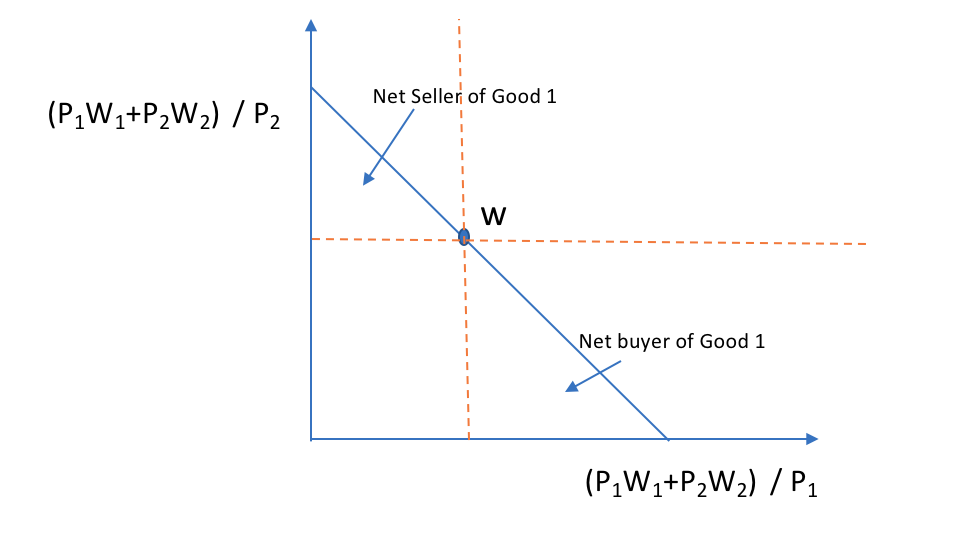
\includegraphics[scale=0.4]{12}
\end{center}
\end{definition}

\section{Intertemporal Choice}
\begin{itemize}
\item Consumption decisions have \underline{dynamic} component: must decide \underline{what}, but also \underline{when} to consume 
\item We can express dynamic problems as variants of static problems we have covered. 
\item Consider an economy with 2 periods
\item There is a single consumption good in each period and let \(c_1, c_2 geq 0\) denote consumption choices in periods 1 and 2 
\begin{itemize}
\item Suppose price of consumption good is \(p > 0\) in each period. 
\item Consumer has income \(m_1 > 0\) in period 1 and \(m_2 > 0\) in period 2.
\item Any unspent income from period 1 can be saved at interest interest rate \(r\) [Saving \([m_1 - pc_1]\) yields \((1+r)[m-p_1c_1]\) in period 2
\item Intertemporal budget set with saving is 
\[B = \{(c_1, c_2) \in \mathbb{R}^2_+ \mid  p_1c_1 \leq m_1 \hspace{0.1cm} , p_2c_2 \leq m_2 + (1+r) [m_1 - pc_1]\}\]
\end{itemize}
\end{itemize}

\begin{center}
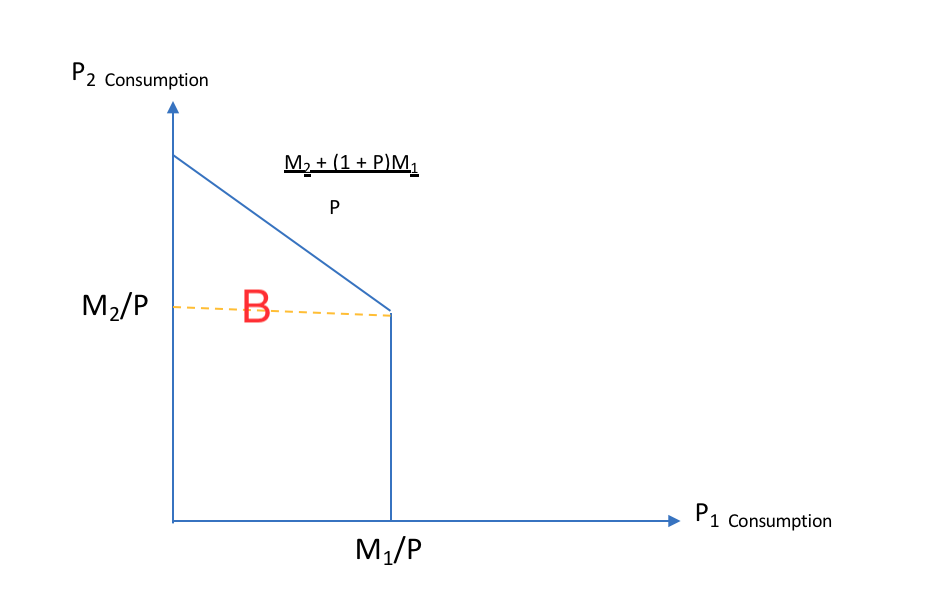
\includegraphics[scale=0.4]{13}
\end{center}


\end{document}





